%Methodenwahl % Begründung der Auswahl

Industrieroboter können eine Vielzahl von verschiedenen Aufgabengebieten übernehmen. Die Aufgabengebiete reichen hierbei von Bedinungs- über Bearbeitungs- bis hin zu Montageabläufen \cite{noauthor_industrieroboter_2020}. Die Schwierigkeit besteht hierbei zunächst die Anforderungen an den erforderlichen Industrieroboter zu definieren und wenn möglich einzugrenzen. Da die Kommunikation mit und ohne ROS getestet werden soll ist es von Vorteil einen Industrieroboter mit einer bereits vorhandenen ROS-Unterstützung zu verwenden. Zudem ist es erforderlich den Industrieroboter über eine direkte Schnittstelle ansprechen zu können um die gewünschten Abläufe, welche geteacht werden sollen, mit einer direkten Kommunikation ohne Netzwerklatenzen testen und einen Vergleich auf Grund des Zeitverhaltens anstellen zu können. Die Interoperabilität mit Simulationsumgebungen ist auch abzuwägen, da die Tests mithilfe einer Simulationsumgebung ohne Sicherheitsbedenken für die bedienende Person durchgeführt werden können und zudem für Regressionstests der Gestenerkennungssoftware praktikabel ohne einen realen Roboter durchgeführt werden können. Im weiteren Verlauf muss zudem die Entscheidung für einen Tiefensensor durchgeführt werden um eine Gestenerkennung, welche zur Steuerung des Inustrieroboters eingesetzt werden soll, realiseren zu können. Bei der Gestenerkennung steht vor allem die Ergonomie und die Sicherheit der bedienenden Person im Vordergrund. Hierbei muss unter anderem beachtet werden, dass zufällige Gesten nicht als Aktion gewertet werden, da dies ansonsten die Sicherheit der bedienenden Person negativ beinflussen kann. Bei der Programmiersprache und Programmierumgebung ist dabei darauf zu achten, dass diese zu ROS kompatibel ist, da ansonsten erheblicher Mehraufwand bei der Umsetzung entstehen würde.


\section{Industrieroboter}
Ein Industrieroboter ist ein universell einsetzbarer Bewegungsautomat, welcher im industriellen Einsatzgebiet eingesetzt wird. Zu erwähnen ist, dass Industrieroboter zumeist auf ein bestimmtes Problem zugeschnitten sind. Aus diesem Grund werden diese je nach der Positionsgenauigkeit, Tragfähigkeit, Arbeitsbereich, Arbeitsgeschwindigkeit und maximaler Reichweite unterschieden. Die maximale Reichweite ist bei ortsfesten Industrierobotern durch die Armlänge und die Freiheitsgrade begrenzt. Im Gegensatz zu ortsfesten Industrierobotern können bewegliche Industrieroboter sich zusätzlich in der Umgebung bewegen und werden daher durch die Bewegungsvorrichtung begrenzt \cite{noauthor_industrieroboter_2020}.

\begin{figure}[htb]
	\centering
	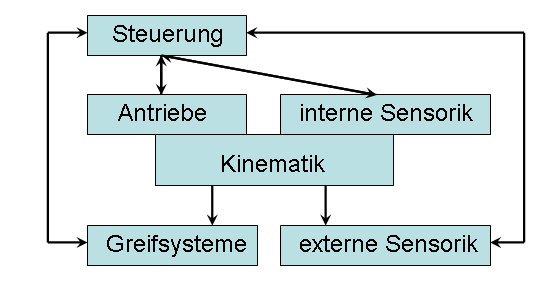
\includegraphics[width=0.6\textwidth]{images/stand_der_technik/Struktur_IR}
	\caption[Struktur eines Industrieroboters]{Struktur eines Industrieroboters \\Quelle: \cite{noauthor_industrieroboter_2020}}
	\label{fig:struktur_eines_industrieroboters}
\end{figure}
\FloatBarrier

Wie in Abbildung \ref{fig:struktur_eines_industrieroboters} zu sehen ist, besteht ein Industrieroboter grundlegend aus einem Roboterarm, welcher auch Manipulator genannt wird, einer Steuerungseinheit, welche für die Überwachungung und Übersetzung der Aktionen auf den spezifischen Industrieroboter zuständig ist und einem Endeffektor, welcher über ein Greifsystem befestigt wird. Über den Manipulator, welcher Gelenke und Antriebe aufweist, wird die Kinematik realisiert, welche es ermöglicht den Manipulator im Raum zu bewegen. Um jeden Punkt im 3D-Raum ansteuern zu können sind mindestens 3 DOF erforderlich, welche über Gelenke realisiert werden. Um jeden Punkt im Raum mit jeder beliebigen Orientierung ansteuern zu können benötigt es jedoch 6 DOF, wobei 3 Gelenke für translatorische und weitere 3 Gelenke für rotatorische Bewegungsabläufe zuständig sind. Der Endeffektor kann auf verschiedene Arten realisiert werden. Zumeist ist es jedoch ein Werkzeug, welches z.B. für Schweiß-, Bohr-, Beschichtungs-, Klebe-, Montage- und Schneidearbeiten eingesetzt werden kann. Da der Endeffektor austauschbar ist, besteht jedoch aber auch die Möglichkeit einen Greifer oder einen anderen spezifisch für eine Aufgabe konzipierten Endeffektor zu montieren und zu verwenden. Damit die Steuerungseinheit die Gelenkpositionen und Antriebsgeschwindigkeiten ermitteln kann sind zudem Messsysteme erforderlich, welche als interne Sensoren bezeichnet werden. Als optionale Komponente können zudem externe Sensoren beim Industrieroboter verbaut sein, welche unter anderem zur Ermittlung von Objektposition im 3D-Raum und deren Größe verwendet werden können. Je nach Arbeitsumfeld kann es auch erforderlich sein, dass ein System zum Wechseln der Endeffektoren eingesetzt wird um mehrere Arbeitsschritte mit einem einzigen Industrieroboter durchführen zu können \cite{hagele_aufbau_2006}.

\subsection{Bauformen}
Industrieroboter können entweder zur seriellen oder parallelen Kinematik zugeordnet werden. Der Unterschied besteht darin, dass die Achsen bei der seriellen Kinematik seriell angeordnet sind, wohingegen bei der paralleln Kinematik die Achsen parallel angeordnet werden.

\begin{figure}[htb]
	\centering
	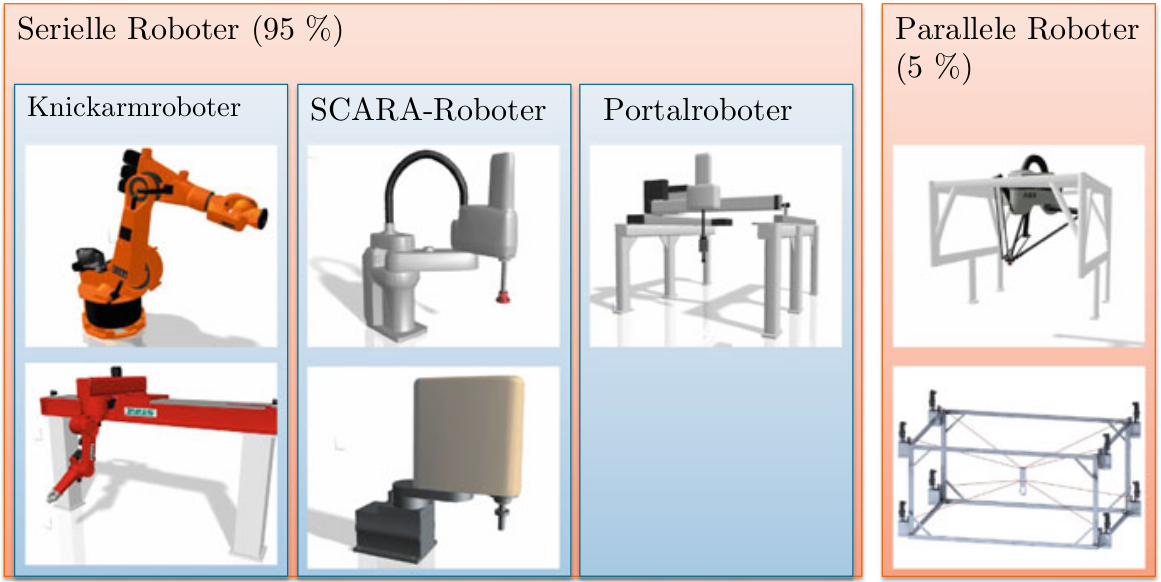
\includegraphics[width=0.9\textwidth]{images/stand_der_technik/bauformen_industrieroboter}
	\caption[Bauformen von Industrierobotern]{Bauformen von Industrierobotern \\Quelle: \cite[18]{pott_industrielle_2019}}
	\label{fig:bauformen_industrieroboter}
\end{figure}
\FloatBarrier

Mit 95\% Anteil haben sich Industieroboter mt serieller Kinematik aufgrund ihrer Bauweise und den bei Knickarmrobotern sehr großen Bewegungsfreiheit durchgesetzt, wie aus der Abbildung \ref{fig:bauformen_industrieroboter} zu entnehmen ist. Nur ein geringer Teil von 5\% der Industrieroboter besitzen eine parallele Kinematik, zu denen unter anderem der Delta- und Seil-Roboter zählen. In der Abbildung \ref{fig:bauformen_industrieroboter} ist der Delta-Roboter im Bereich der parallen Roboter oben und der Seilroboter im unteren Bereich zu sehen. Die parallele Kinematik zeichnet sich dabei durch mindestens eine geschlossene kinematische Kette aus. Zu den seriellen Industrierobotern zählen unter anderem Knick-, SCARA- und Portal-Roboter und alle anderen Roboter, welche eine offene kinematische Kette aufweisen. Industieroboter mit serieller Kinematik zählen zu den am weitest verbreitesten Industrierobotern. Im Gegensatz zu den seriellen Industrierobotern bieten parallele Industrieroboter durch die direkte Verbindung zum Greifsystem den Vorteil, dass die nachfolgenden Glieder und deren Massen nicht wie beim seriellen Industrieroboter die Dynamik des Systems beeinflussen. Dies führt dazu, dass eine sehr hohe Genauigkeit und eine sehr hohe Steifigkeit garantiert werden kann. Zudem sind durch die parallele Kinematik hochpräzise Ansteuerungsmanöver mit sehr hoher Geschwindigkeit durchführbar. Der Nachteil besteht jedoch darin, dass der parallele Industrieroboter ortsfest ist. Die parallele Kinematik zählt daher eher zur Ausnahme und wird aus diesem Grund vermehrt für Pick-and-Place-Aufgaben oder Sondermaschinen eingesetzt, wo Geschwindigkeit, eine hohe Präzision und hohe Dynamik erforderlich ist \cite[17\psqq]{pott_industrielle_2019}.\\

Der Knickarmroboter, welcher zu den seriellen Industrierobotern zählt und zumeist 6 DOF aufweist, bietet den Vorteil, dass dieser für weitere Bewegungsfreiheit auf eine zusätzliche Linearachse montiert werden kann. Dadurch ist es unter anderem Möglich verschiedene Arbeitspositionen eines großen Objekts ansteuern zu können. Da der Knickarmroboter eine armartige Form aufweist, ist dieser zumeist für schwer erreichbare Stellen geeignet. Aufgrund der offenen kinematischen Kette und der Möglichkeit einer sehr großen Nutzlast leidet jedoch die Absolutgenauigkeit darunter. Typischwerweise werden Knickarmroboter für Schweiß-, Handhabungs- und Klebearbeiten eingesetzt. Eine weitere Möglichkeit um serielle Industrieroboter zu realisieren stellen die SCARA-Roboter dar. Diese weisen im Gegensatz zu den Knickarmrobotern weniger Freiheitsgrad. Typischwerweise werden zumeist 3 oder 4 DOF verbaut, wodurch die Bewegungsfreiheit eingeschänkt wird. Zudem sind aufgrund der Bauform nur geringere Arbeitslasten und kleinere Arbeitsbereiche nutzbar. Dies zeigt sich auch beim Aufgabenbereich, welcher großteils in der Montage und Pick-and-Place besteht. Portale, welche auch zu den seriellen Industrierobotern zählen, können sehr hohe Nutzlasten und große Bewegungen durchführen. Sie sind nach den Knickarmrobotern die zweithäufigste Bauform. Zu den Aufgabengebieten zählen Pick-and-Place, Maschinenbestückungen und Kommisionsarbeiten \cite[17\psqq]{pott_industrielle_2019}.

\subsection{Positions- und Bahngenauigkeit}
Um Genauigkeitsmessungen an einem Industrieroboter durchzuführen ist es erforderlich die spezifischen Genauigkeiten eines Industrieroboters zu kennen und diese in einen Zusammenhang zu bringen. Bei Industrierobotern ist die Genauigkeit in sehr vielen Aufgabenbereichen, wie z.B Laserschneiden oder Schweißen, sehr entscheident. Eine hohe Genauigkeit spart Kosten und Zeit ein, da eine teure und zeitintensive Nachbearbeitung entfällt. Aus diesem Grund ist es entscheident, dass der Industieroboter für spezielle Aufgabenbereiche eine hohe Positions- und Bahngenauigkeit aufweist. Um die Positions- und Bahngenauigkeit von Industrierobotern beurteilen zu können verwendet man die Absolut- und Wiederholgenauigkeit. Beide Kennwerte beschreiben die Qualität der Übereinstimmung der Realität und des Modells und sind in der ISO 9283, welche die Robotergenauigkeit beinhaltet und beschreibt, standardisiert \cite[28\psqq]{pott_industrielle_2019}.

\begin{figure}[htb]
	\centering
	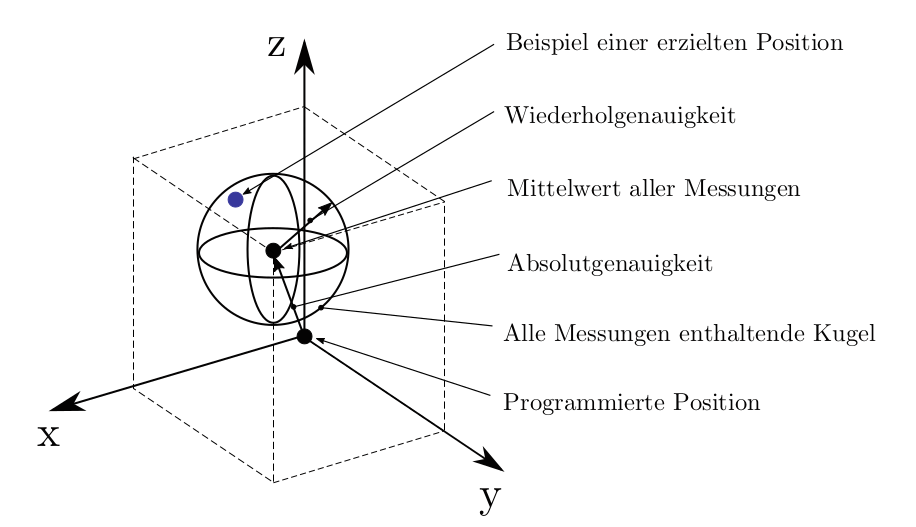
\includegraphics[width=0.686\textwidth]{images/stand_der_technik/absolutgenauigkeit_und_wiederholgenauigkeit}
	\caption[Absolut- und Wiederholgenauigkeit]{Absolut- und Wiederholgenauigkeit \\Quelle: \cite[29]{pott_industrielle_2019}}
	\label{fig:absolutgenauigkeit_und_wiederholgenauigkeit}
\end{figure}
\FloatBarrier

In der Abbildung \ref{fig:absolutgenauigkeit_und_wiederholgenauigkeit} ist der Zusammenhang zwischen der Absolut- und Wiederholgenauigkeit zu erkennen. Die Wiederholgenauigkeit wird ermittelt indem der Industrieroboter über mehrere Zyklen hinweg immer wieder die gleiche Pose anfährt. Hierbei beeinflussen systematische Gegebenheiten, wie z.B. termische Ausdehnung durch Umgebungstemperatur, sowie aber auch durch die Motorwärme, Justagefehler der Achsen, Fertigungstoleranzen oder sogar Kollisionen die Genauigkeit des Gesamtsystems um die Zielpose exakt ansteuern zu können. Aus diesen Gründen ist es empfehlenswert den Industrieroboter jährlich auf die Genauigkeit zu prüfen und gegebenenfalls zu justieren. Im Gegensatz zur Wiederholgenauigkeit beschreibt die Absolutgenauigkeit wie genau der Industrieroboter eine theretisch programmierte Zielpose, z.B. mittels CAD-Software erlernt, im Bezug zum Roboterkoordinatensystem ansteuern kann. Standardmäßig beträgt die Wiederholgenauigkeit bei Industrierobotern \num{0,1} mm wohingegen die Absolutgenauigkeit standardmäßig eine maximale Abweichung von 1 mm aufweist \cite[28\psqq]{pott_industrielle_2019}.

\begin{figure}[htb]
	\centering
	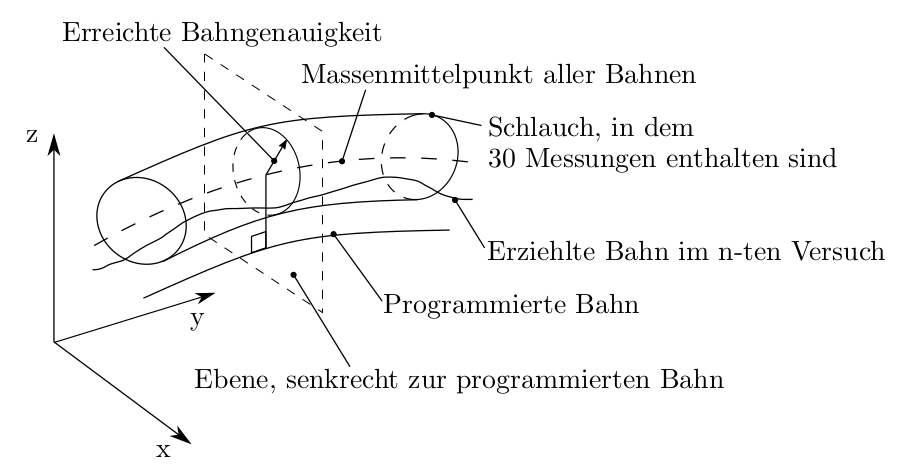
\includegraphics[width=0.735\textwidth]{images/stand_der_technik/bahngenauigkeit}
	\caption[Bahngenauigkeit]{Bahngenauigkeit \\Quelle: \cite[30]{pott_industrielle_2019}}
	\label{fig:bahngenauigkeit}
\end{figure}
\FloatBarrier

Bei einer großen Abweichung der Absolutgenauigkeit führt dies jedoch zu einem schlechten erreichen der Zielpose und dadurch auch zu einem schlechten Bahnverhalten wie in Abbildung \ref{fig:bahngenauigkeit} durch die erzielte Bahn im n-ten Versuch ersichtlich ist. Die erzielte Bahn weist deutliche Schwingungen auf und weicht daher erkennbar von der programmierten Bahn ab. Aus diesem Grund bieten viele Hersteller gegen einen Aufpreis absolutvermessene Industrieroboter an um diesen Genauigkeitsfehler zu kompensieren \cite[29\psq]{pott_industrielle_2019}. Wenn eine sehr hohe Wiederholgenauigkeit gewünscht ist kann auch mit Spezialrobotern eine Wiederholgenauigkeit von bis zu 1 \si{\micro}m erreicht werden \cite{noauthor_genauigkeit_nodate}.

\begin{figure}[htb]
	\centering
	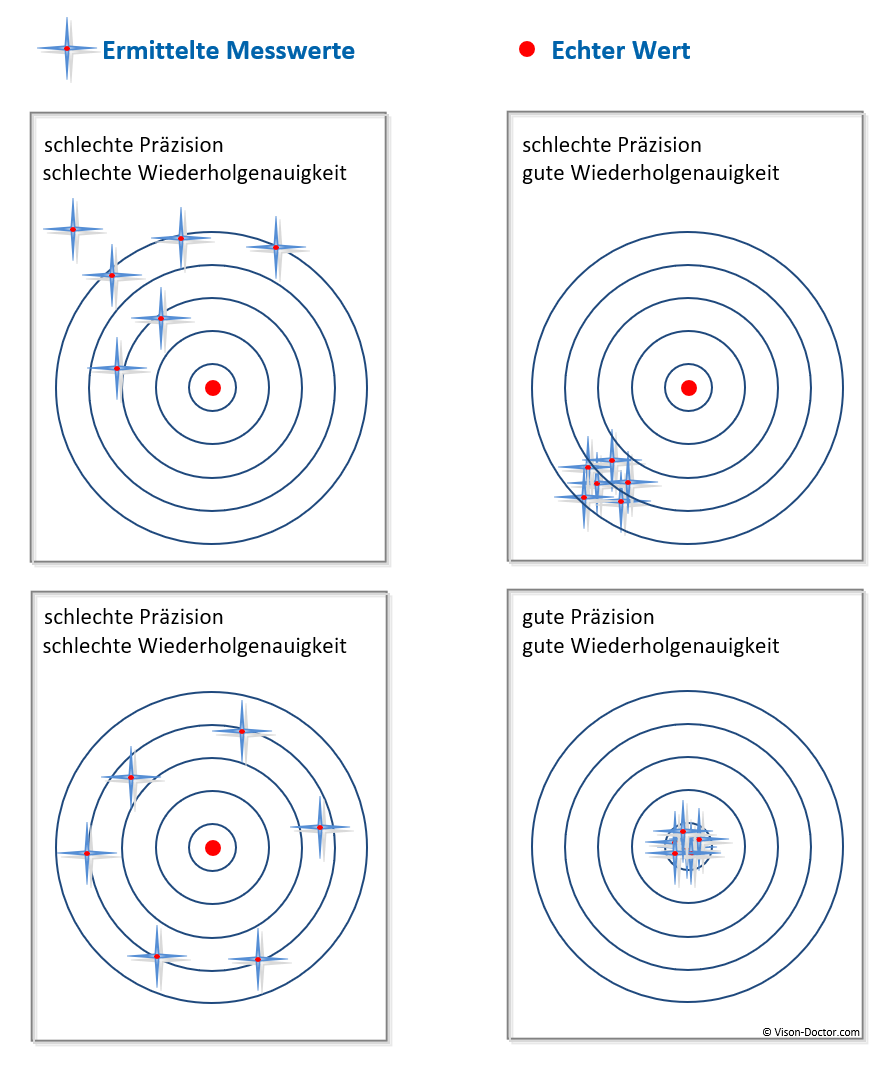
\includegraphics[width=0.57\textwidth]{images/stand_der_technik/wiederholgenauigkeit}
	\caption[Wiederholgenauigkeit]{Wiederholgenauigkeit \\Quelle: \cite{noauthor_prazision_nodate}}
	\label{fig:wiederholgenauigkeit}
\end{figure}
\FloatBarrier

Wie in Abbildung \ref{fig:wiederholgenauigkeit} zu sehen ist, kann daraus geschlossen werden, dass keine hohe Präzision durch eine schlechte Wiederholgenauigkeit möglich ist. Aus diesem Grund kann auch gesagt werden, dass die Wiederholgenauigkeit entscheidenter als die Absolutgenauigkeit zum erreichen der Zielposition ist, da umgekehrt nicht gesagt werden kann, dass eine hohe Präzision durch eine gute Wiederholgenauigkeit erreicht wird \cite{noauthor_genauigkeit_nodate}.


%"Die genaue Definition findest Du in der EN ISO 29283 (ehemals ISO 9283). Dort wird auch beschrieben, wie man die Genauigkeiten ermittelt." (https://www.roboternetz.de/community/threads/35643-absolutgenauigkeit)



% ----------------------

% S. 25 pott_industrielle_2019   kinematische Transformation (direkte & indirekte Transformation)
% cBei seriellen Robotern ist die direkte Kinema- tik stets eindeutig, während es für eine gewünschte Position des Endeffektors häufig mehr als eine Lösung gibt. Bei Knickarmrobotern kann es je nach Position bis zu acht mögliche Achsstellungen für eine vorgegebene Position des Endeffektors geben.``



% S. 54 - 56 pott_industrielle_2019

%\subsection{Bewegungsdynamik}
%\subsection{Steifigkeit}




% https://www.youtube.com/watch?v=wKiJaK-RDKI
% https://www.youtube.com/watch?v=GNrU2zviRpc
% https://www.youtube.com/watch?v=A9M1zX3GzX0
% https://www.youtube.com/watch?v=9iCLK__7ymY



% https://de.wikipedia.org/wiki/Industrieroboter
% https://link.springer.com/chapter/10.1007%2F3-540-34823-9_27

% Wie schnell können diese reagieren? (Zeitverhalten) je nach Roboterarm verschieden


\section{Teachen von Industrierobotern}
Teachen, welches auch als Teach-In bezeichnet wird, ist eine von mehreren möglichen Varianten einem Industrieroboter gewünschte Posen beizubringen, damit dieser seine Arbeitsaufgabe autonom durchführen kann.

\subsection{Offline- und Online-Programmierverfahren}
Unterschieden wird bei den Lernmethoden zwischen Offline- und Online-Programmierverfahren. Die am weitest verbreitesten Offline-Methoden sind die textuelle Programmierung und das Erlernen mit einer CAD-Software. Bei der textuellen Programmierung ist es notwendig über ausreichend Programmierkenntnisse in der Programmiersprache des Industieroboter-Herstellers oder einer kompatiblen Programmiersprache zu verfügen, wohingegen bei einer CAD-Software einem virtuellen Industrieroboter in einer virtuellen Umgebung die Posen beigebracht werden können. Beide Methoden benötigen im Vergleich zum Teachen sehr viel mehr Vorwissen und sind daher nur nach erheblichem Lernaufwand nutzbar. Das Teachen zählt neben der Playback-Methode, welches ein direktes Führen des Roboterarms ermöglicht, zu den Online-Programmierverfahren. Beim Teachen kommt eine Steuerkonsole zum Einsatz mit deren Hilfe es möglich ist dem Industieroboter Posen beizubringen. Zuerst wird eine Pose mit mehreren aufeinander folgenden Steuerungsbefehlen angefahren. Anschließend, wenn eine gewünschte Pose erreicht wurde, kann diese einzelne Pose per Steuerungsbefehl in der Steuerungseinheit gespeichert werden. Das Anfahren und Speichern der Posen wird solange wiederholt bis die gesamte Arbeitsaufgabe dem Industrieroboter beigebracht wurde. Wenn notwendig, können im Nachhinein die gespeicherten Posen korrigiert werden um eine höhere Genauigkeit zu erzielen oder um Fehler zu korrigieren. Im Gegensatz zum Teachen wird beim Playback-Verfahren genau die Bewegung gespeichert, welche durch das direkte Führen des Roboterarms entsteht, und beim Ausführen der Arbeitsaufgabe auf die gleiche Weise wiederholt \cite{noauthor_industrieroboter_2020}. Beim Teachen hingegen kann zwischen den Punkten die Geschwindigkeit, Beschleunigung und sogar die Art des Pfades eingestellt werden. Bei der Art des Pfades kann frei zwischen Point-to-Point und Continuous Path gewählt werden. Point-to-Point erzwingt den für den Industrieroboter geometrisch günstigsten Pfad zwischen den Punkten zu wählen, welcher normalerweise keine gerade lineare Bahnbewegung darstellt und daher zu einem unbekannten Pfad führt. Bei Continuous Path wird hingegen von einem Punkt direkt zum nächsten Punkt entlang eines vordefinierten Pfades gefahren, welcher z.B. eine gerade lineare oder eine durch einen Hilfspunkt erzeugte kreisförmige Bahnbewegung sein kann. Durch diese Einstellungsmöglichkeiten ist es beim Teachen möglich noch höhere Genauigkeiten als bei der Playback-Methode zu erzielen. Im Gegenzug steigt durch die höhere Genauigkeit, aber auch der Programmieraufwand, da für eine hohe Genauigkeit viele Zwischenpunkte gelernt werden müssen \cite{noauthor_teach-technik_2020}.\\

Für alle Programmierverfahren, ob Offline- oder Online-Programmierverfahren, welche zur Programmierung von Industrierobotern eingesetzt werden, kann gesagt werden, dass sie einen gewissen Lernaufwand bei der Einarbeitung benötigen. Der Lernaufwand um ein Programmierverfahren zu erlernen sinkt jedoch erheblich für untrainierte Personen, wenn eine visuelle Lernmethode eingesetzt wird. In Zukunft besteht daher ein sehr großes Potenzial zur Erforschung und Verbesserung von Gesten, Sprach und visuellen Systemen, da diese Systeme eine für den Menschen vertrauliche Interaktionsmöglichkeit bieten \cite{biggs_survey_nodate}.

\subsection{Teach Pendant}
\begin{figure}[htb]
	\centering
	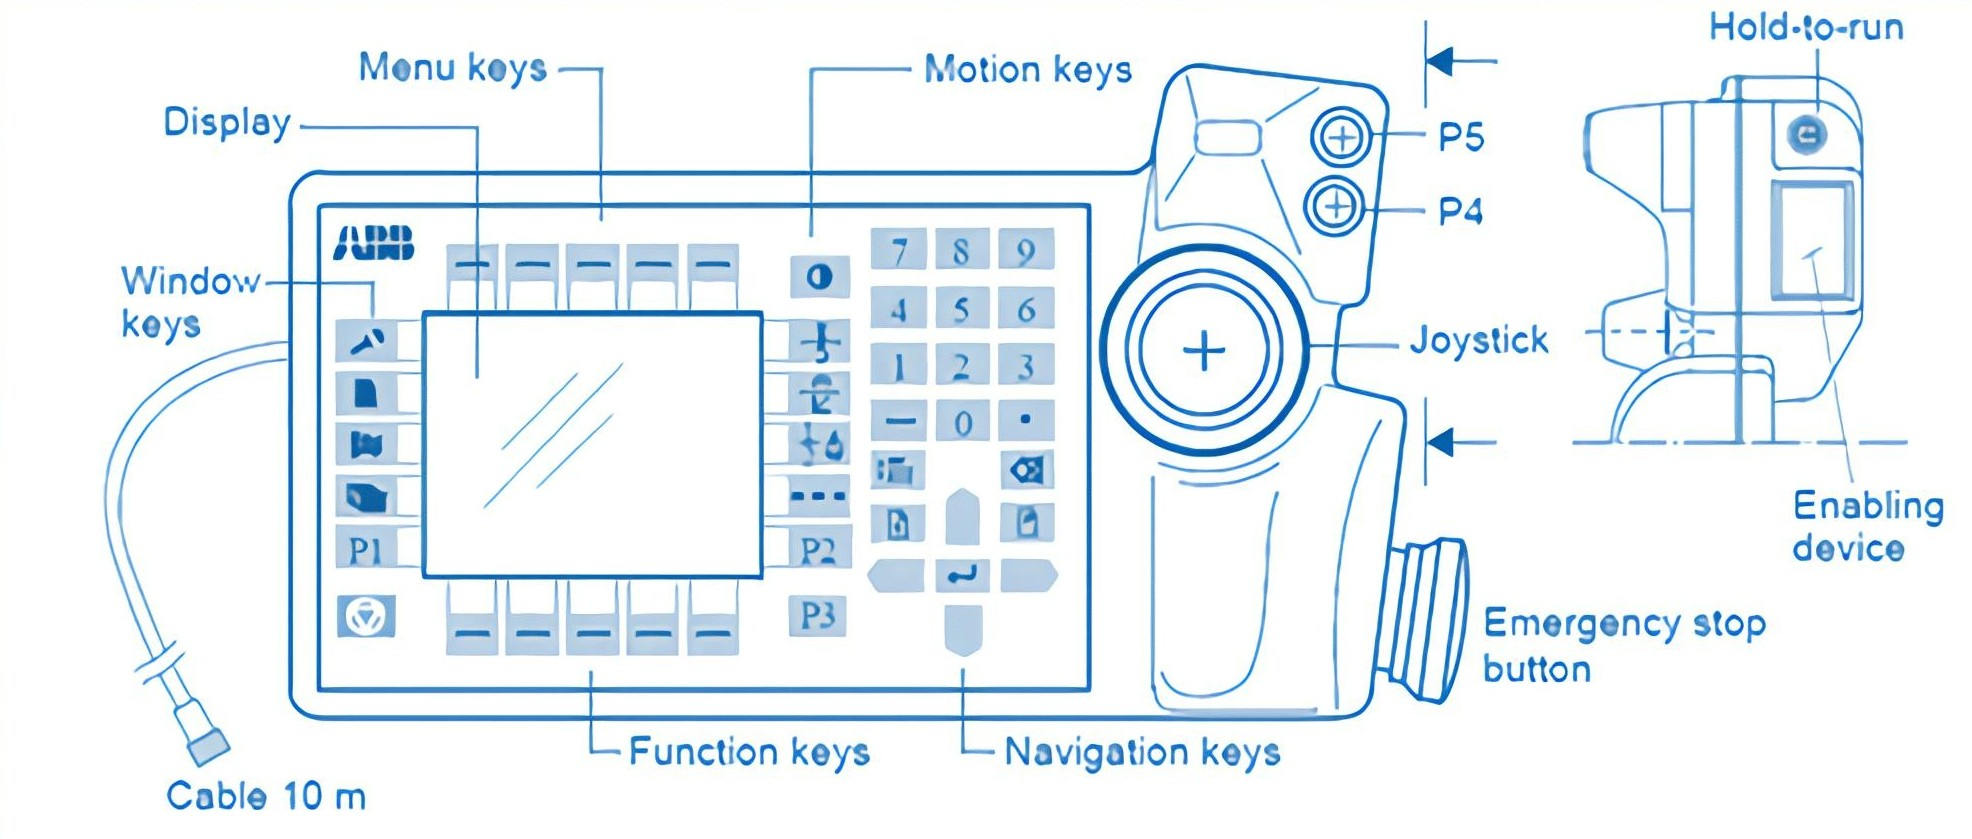
\includegraphics[width=0.715\textwidth]{images/stand_der_technik/teach_pendant}
	\caption[Teach Pendant im Querformat von ABB]{Teach Pendant im Querformat von ABB \\Quelle: \cite{noauthor_programengif_nodate}}
	\label{fig:teach_pendant}
\end{figure}
\FloatBarrier

Zur Programmierung mit dem Teach-In-Verfahren werden Teach Pendants, wie in Abbildung \ref{fig:teach_pendant} zu sehen, eingesetzt, welche im Gegensatz zu früheren Modellen je nach Hoch- oder Querformat im oberen oder im linken Bereich des Teach Pendants über ein Display mit oder ohne Touch-Funktionalität verfügen \cite{nof_handbook_1999}. Unterschieden wird bei den herstellerspezifischen Teach Pendants zwischen dem Hoch- und Querformat. Beim Hochformat wird das Teachpendant mit beiden Händen gehalten und mithilfe der Daumen werden die Knöpfe betätigt. Im Gegensatz zum Hochformat ist in einem Teach Pendant mit Querformat ein größeres Display verbaut und das Teach Pendant kann im Querformat mit beiden Händen oder nur mit der linken Hand gehalten werden. Die rechte Hand kann dazu verwendet werden Eingaben auf dem Teach Pendant zu tätigen oder mittels des verfügbaren 3 DOF Joysticks oder 6 DOF 3D-Maus zum Steuern des Industrieroboters verwendet werden. Beim Betätigen des Joysticks oder der 3D-Maus reagiert der Industrieroboter bereits bei sehr feinen Bewegung des Eingabegerätes mit einer entsprechenden Bewegung in die jeweilige vorgegebene Richtung. Je weiter der Joystick oder die 3D-Maus in eine Richtung bewegt wird, desto schneller bewegt sich auch der Industrieroboter in die ensprechende Richtung \cite{prassler_advances_2004}. Jedes Teach Pendant muss einen Notstop-Schalter aufweisen um die Maschine und das Teach Pendant jederzeit außer Betrieb setzen zu können. Dieser Notstop-Schalter ist zumeist rechts oben oder rechts unten, wie in Abbildung \ref{fig:teach_pendant} zu sehen ist, als große rote Taste realisiert. Als weitere Schutzvorkehrung muss das Teach Pendant einen \quoteMark{Enable device}-Schalter aufweisen. Der \quoteMark{Enable device}-Schalter wird Umgangssprachlich Dead man's switch genannt und muss während die Maschine bedient wird ununterbrochen gehalten werden. Dabei ist zu beachten, dass wenn der Notstop-Schalter losgelassen oder zu fest gedrückt wird, der Industrieroboter zum Anhalten gebracht wird. Das Teach Pendant geht davon aus, dass wenn dieser Schalter zu fest gedrückt oder losgelassen wird, dass die Person, welche die Kontrolle über das Teach Pendant hat bewusstlos, Tod oder sogar nicht mehr an der Maschine ist. Durch das Auslösen dieses Sicherheitsschalters wird der Industrieroboter zum Anhalten gebracht und weiterer Schaden und gefährliche Situationen werden verhindert \cite{noauthor_dead_man_switch_2020}.\\

Weitere Tasten wie z.B. Menü, Funktionen, Bewegung und Navigation, wie in Abbildung \ref{fig:teach_pendant} zu sehen ist, sind herstellerspezifisch und daher optional. Aus diesem Grund kann ein Teach Pendant je nach Hersteller unterschiedliche herstellerspezifischen Funktionstasten aufweisen, welche zumeist Zugriff auf die am häufigsten verwendeten Funktionalitäten des Teach Pendants bieten \cite{dinwiddie_basic_2015}. Neben diesen Sicherheitsfeatures gibt es auch herstellerübergreifende Features um den Industrieroboter zu steuern. Eines dieser Features ist das Wechseln zwischen unterschiedlichen Bewegungsmodi. Zu diesen Bewegungsmodi zählen der Gelenk-, Welt-Koordinatensystem- und Tool-Koordinatensystem-Modus. Der Gelenk-Modus erlaubt es die Position der Gelenke mithilfe des Teach Pendants jeweils einzeln oder alle Gelenke zusammen zu bewegen. Dieser Modus ermöglicht es daher die volle Kontrolle über alle Gelenke des Industrieroboters zu erlangen und diese an die jeweiligen Gegebenheiten der Umgebung anzupassen. Der Gelenk-Modus wird daher häufig zum Erreichen von schwer zugänglichen Stellen eingesetzt. Im Gegensatz zum Gelenk-Modus erlaubt es der Welt-Koordinatensystem-Modus den Mittelpunkt des Endeffektors (TCP) in der x-, y- oder z-Achse zu bewegen und Rotationen um die x-, y- oder z-Achse im Weltkoordinatensystem durchzuführen. Der Sockel des Industrieroboters stellt den Mittelpunkt des Weltkoordinatensystems dar. Für diesen Modus werden die Positionen der Gelenke über die inverse Kinematik, ermittelt und automatisch vom Teach Pendant eingestellt \cite{noauthor_jogging_2017}. Wenn bei Knickarmrobotern die Pose des Endeffektors bei der Berechnung der inversen Kinematik berücksichtigt wird, kann es je nach gewählter Pose des Endeffektors bis zu acht mögliche Gelenksstellungen für den Knickarmroboter geben, wordurch die inverse Kinematik für diesen Fall nicht mehr eindeutig für die gewählte Pose ist \cite[25]{pott_industrielle_2019}. Die letzte Möglichkeit den Industrieroboter einzustellen besteht darin, den TCP des Industrieroboters im Tool-Koordinatensystem-Modus einzustellen. Der Tool-Koordinatensystem-Modus besitzt die gleichen Möglichkeiten, wie der Welt-Koordinatensystem-Modus, verwendet jedoch aber als Referenzkoordinatensystem den TCP \cite{noauthor_jogging_2017}.

% Genauigkeit % TODO: Welche Genauigkeit ist mit einem Teach Pendant möglich?


% Überschleifen: https://www.xplore-dna.net/mod/page/view.php?id=451

% Robotersteuerung (Bewegungsbahn): https://wiki.induux.de/Robotersteuerung

% Point-to-point: https://www.youtube.com/watch?v=Fd7wjZDoh7g

% https://www.computerwoche.de/a/mikroprozessoren-machen-programmierung-erst-effektiv,1160823


\section{Arten von Echtzeitverhalten}
Im Umgang mit Industrierobotern ist es notwendig Echtzeitsysteme einzusetzen, welche für den jeweiligen spezifischen Anwendungsfall die Anforderung an die Reaktionszeit des Systems sicherstellen. Die Anforderung an das Echtzeitsystem können vielseitig sein. Diese können bei sehr zeitkritischen und sicherheitsrelevanten Systemem wenige Millisekunden und bei weniger relevanten Aufgaben, wie z.B. das Speichern von Daten auf eine Festplatte, bis hin zu mehreren Minuten, Stunden, Tagen oder sogar länger in Anspruch nehmen. Die entscheidente Herausforderung für das Echtzeitsystem ist es deshalb zu garantieren, dass das Ergebnis in dem für den Anwendungsfall erforderlichen Zeitintervall berechnet wird. Die Zeitintervalle werden durch die Hardware limitiert, wordurch eine für den Anwendungsfall entsprechend schnelle Hardware erforderlich ist. Anwendungsfälle mit genügend kleinen Zeitinvervallen können daher nur mit entsprechend schneller Hardware realisiert werden \cite{noauthor_echtzeitsystem_2020}.\\

Bei Echtzeitsystemen wird zwischen harter, fester und weicher Echtzeitanforderung unterschieden. Unter harter Echtzeitanforderung versteht man, dass das Ergebnis der Berechnung innerhalb des Zeitintervalls  erfolgen muss, da ansonsten das System versagt hat. Bei Nichteinhaltung des Zeitintervalls besteht ansonsten die Möglichkeit, dass es zu einem Schaden kommt. Als Beispiel kann die Notbremsung eines autonom fahrenden Autos eine harte Echtzeitbedingung darstellen. Im Gegensatz zur harten Echtzeitanforderung stellt die feste Echtzeitanforderung eine etwas entspanntere Echtzeitanforderung dar. Bei der festen Echtzeitanforderung wird davon ausgegangen, dass kein unmittelbarer Schaden zustande kommt. Daher kann das Zeitintervall auch überschritten werden. Das Ergebnis wird beim Überschreiten des Zeitintervalls jedoch zumeist ungültig und weitere darauf aufbauende Berechnungen können daher abgebrochen werden. Ein Beispiel für eine feste Echtzeitanforderung kann sein, dass die derzeitige Position eines Fahrzeugs nach dem Weiterbewegen des Fahrzeugs nicht mehr die gleiche Position ist und Berechnungen auf diesen Daten schlicht zu falschen Ergebnissen führen würden. Aus diesem Grund würde es keinen Sinn machen mit den veralteten Daten weiterzuarbeiten. Bei weichen Echtzeitanforderung ist das Zeitintervall für die Bearbeitung der Aufgabe als Vorgabe zu sehen und kann wenig oder sehr stark überschritten werden. Zum Beispiel bei Multimediasystemen führen geringe Überschreitungen des Zeitintervalls zu verzögerten Bildern, welches jedoch in einem gewissen Rahmen  \cite[321\psq]{worn_echtzeitsysteme_2006} \textcolor{red}{TODO:}.

% Echtzeitkernel
% deterministisches & nicht deterministisches Zeitverhalten


% https://de.wikipedia.org/wiki/Echtzeitsystem
% Linux benötigt einen speziellen Kernel, FreeBSD, MacOSX Kernel, Windows NT Kernel (die am häufigsten verwendeten Betriebssysteme


% Deadlock verhindern: https://de.wikipedia.org/wiki/Deadlock_(Informatik)

% https://books.google.at/books?id=llghBAAAQBAJ&pg=PA182&lpg=PA182&dq=zeitverhalten+echtzeitverhalten&source=bl&ots=hVS6os93-J&sig=ACfU3U3Yt0ChDwoIIZzmuAYv63MRfg-Y6Q&hl=de&sa=X&ved=2ahUKEwj8qvuqzerpAhVp5KYKHZTBA0AQ6AEwBHoECAgQAQ#v=onepage&q=zeitverhalten%20echtzeitverhalten&f=false
% --> downloaded
% S. 1 - 4
% Echtzeitbetriebssysteme: S. 343, 420, 425
% Arten: S. 318 - 322


% 'Eine Gruppe mit ständig wachsenden Funktionen hat geringe Echtzeit-
% Anforderungen ( 100 ms bis Sekunden ), wie Roboterprogrammarchivierung,
% Benutzerschnittstellen, SPS-Programmierung, Kommunikation zum Leitrechner,
% Ferndiagnose, Robotersimulation, Bedienungsanleitungen in verschiedenen Spra-
% chen, Inbetriebnahmehilfen, Auto-Tuning, Tools für Tests und Fehlersuche und
% Lernprogramme.
% Für diese Funktionen bietet ein Standardbetriebssystem (SBS) eine optimale
% Plattform. Die meisten Funktionen lassen sich kostengünstig am weltweiten Soft-
% ware-Markt ohne Entwicklungsaufwand beziehen, z.B. Software für SPS-Pro-
% grammierung, Kommunikation z.B. Ethernet-TCP/IP, Robotersimulation. Für an-
% dere Funktionen wie Benutzerschnittstellen und Hilfen existieren leistungsfähige
% Entwicklungstools.
% Die zweite Gruppe umfasst die eigentlichen Roboterfunktionen wie Interpre-
% ter, Bewegungssteuerung, Technologiesteuerung, Sensor-Datenverarbeitung oder
% Feldbusse für die hohe Echtzeitfähigkeit mit Deadlines von 1 ms bis 10 ms ge-
% fordert sind. Für Antriebsregelungen muss die Gleichzeitigkeit der Regelung ein-
% zelner Achsen mit einem Jitter kleiner 1 μs gewährleistet sein. Hier ist ein leis-
% tungsfähiges Echtzeitbetriebssystem (EBS) mit preemptivem Multitasking und
% kleiner Taskwechselzeit erforderlich.'
% S. 518


% Garbage Collector
% https://de.wikipedia.org/wiki/Echtzeitsystem
% Rechner zur Steuerung von technischen Einrichtungen oder Prozessen wie Maschinen, verfahrenstechnischen Anlagen oder Verkehrsmitteln sind praktisch immer Echtzeitsysteme. 

% Bei einer Software, die Echtzeitbedingungen erfüllen soll, muss die maximale Laufzeit bestimmbar sein und darf keinen nicht oder nur bedingt beeinflussbaren Faktoren unterliegen, muss also deterministisch sein. Dies wird u. a. durch folgende System- oder Softwareeigenschaften beeinflusst: 
% https://de.wikipedia.org/wiki/Echtzeitsystem


% https://books.google.at/books?id=HV-dbKHt0mQC&pg=PA106&lpg=PA106&dq=windows+nt+kernel+not+real+time&source=bl&ots=Gbib90T1TD&sig=ACfU3U0YX16bkZMVXuELZqkmBBchhuNnIQ&hl=de&sa=X&ved=2ahUKEwijjeXH3urpAhUSnVwKHViWD_IQ6AEwA3oECAgQAQ#v=onepage&q=windows%20nt%20kernel%20not%20real%20time&f=false
% "Windows NT kernel is non-preemptable -> no hard RTOS"
% S. 106



% https://de.wikipedia.org/wiki/RTX:_Real_Time_eXtensions_f%C3%BCr_Windows


% Wie lange ist für uns Echtzeit? -> Messungen!



\section{Sicherheitsanforderungen im Umgang mit Industrierobotern}
% Normen, ...

%https://books.google.at/books?id=vGcyKPlZPFEC&pg=PA48&lpg=PA48&dq=teach+pendants+vergleich&source=bl&ots=TPRtrhQPrs&sig=ACfU3U3eokMCgDvbYBbX4ki4KU9tF6B6Jg&hl=de&sa=X&ved=2ahUKEwiyvrqhzOfpAhVlShUIHTCwBu4Q6AEwAXoECAsQAQ#v=onepage&q=teach%20pendants%20vergleich&f=false
% saftey requirements: S. 55
% 50 ms bei WLAN erforderlich


% https://de.wikipedia.org/wiki/Industrieroboter

\section{ROS}
% Aufbauend auf dem Vergleich der Entwicklungsplattformen werden nun die für dieses Projekt am Besten geeigneten Werkzeuge vorgestellt.
% ROS 1 (LTS) vs ROS 2

%https://books.google.at/books?id=llghBAAAQBAJ&pg=PA182&lpg=PA182&dq=zeitverhalten+echtzeitverhalten&source=bl&ots=hVS6os93-J&sig=ACfU3U3Yt0ChDwoIIZzmuAYv63MRfg-Y6Q&hl=de&sa=X&ved=2ahUKEwj8qvuqzerpAhVp5KYKHZTBA0AQ6AEwBHoECAgQAQ#v=onepage&q=zeitverhalten%20echtzeitverhalten&f=false
% 'Deswegen sind lang-
% lebige Softwarearchitekturen mit wiederverwendbaren Bausteinen gefordert.'
% S. 517


\subsection{Architektur}


\subsection{Packages}


\subsection{Zukünftige Entwicklung}
% Community driven, ROS Foundation, ...


\subsection{Anbindungsmöglichkeiten/Interoperabilität}


\section{Simulations- und Testumgebungen}
% Gazebo, vRep, Coppelia Sim, ABB, ...


\section{Tiefensensoren}
% Arten und Vergleich (Vor- und Nachteile)
% Azure Kinect, ...
% Genauigkeit, Techniken, ...

\section{Gesten}
% Mögliche Gesten, Welche Gesten nicht


\section{Ergonomie}


\section{Sicherheit}
% https://de.wikipedia.org/wiki/Industrieroboter
% Maschinenrichtlinien
